\section{Semafori}
I semafori sono uno strumento più avanzato per gestire la cooperazione di più processi.

\spacer
Un semaforo a N valori è una variabile $s$ intera e non negativa sulla quale si può effettuare:
\begin{sitemize}
    \item \textbf{Wait:} decrementa $s$ di 1 se $s>0$, altrimenti sospende il processo. (Oppure \textit{Probeer te verlagen}, P)
    \item \textbf{Signal:} Risveglia uno dei processi in attesa, se nessuno sta attendendo incrementa $s$ di 1. (Oppure \textit{Verhogen} V)
\end{sitemize}

\begin{minted}{java}
wait(S) {
    while(S <= 0) {}; // busy wait
    S--;
}

signal(S) {
    S++;
}
\end{minted}


Definiamo \textbf{Semaforo Contatore} il semaforo a valori in un dominio non limitato. Utile nel controllo di un numero finito di risorse, il semaforo viene inizializzato al numero di risorse disponibili.
\textbf{Semaforo Binario} assume solamente i valori 0 e 1, simile al lock mutex.

\subsection{Implementazione}
L'utilizzo del busy waiting rappresenta un problema per un processo multiprogrammato perché l'attesa spreca cicli di CPU che potrebbero essere usati da un'altro processo.

\spacer
Per risolvere questo problema si può associare ad ogni semaforo una coda di processi in attesa, spesso implementata tramite una queue (First In First Out).


\begin{minted}{java}
struct semaphore {
    int value;
    struct process* list; //puntatore al primo elemento della struttura dati
};

wait(semaphore *S) { 
    S->value--;
    if (S->value < 0) {
        add this process to S->list;
        sleep();
    }
}

signal(semaphore *S) { 
    S->value++;
    if (S->value <= 0) {
        remove a process P from S->list; 
        wakeup(P);
    }
}
\end{minted}

In questo caso $valore$ può essere $<0$, in quelle situazioni $|valore|$ è il numero di processi in attesa.

\subsection{Problemi di Utilizzo}
I semafori possono dare luogo a situazioni inaspettate che devono essere gestite attentamente.

\subsubsection*{Deadlock}
Si possono trovare situazioni in cui uno o più processi attendono risorse che possono essere liberate solo da uno degli altri processi in attesa.

\begin{minipage}{0.45\textwidth}
    \begin{minted}{java}
wait(S);
wait(Q);
...
signal(S);
signal(Q);
\end{minted}
\end{minipage}
\hfill
\begin{minipage}{0.45\textwidth}
    \begin{minted}{java}
wait(Q);
wait(S);
...
signal(Q);
signal(S);
\end{minted}
\end{minipage}

Linux fornisce uno strumento, lockdep, per rilevare i deadlock all'acquisizione di un lock.

\subsubsection*{Starvation}
Gestendo incorrettamente la lista associata al semaforo, per esempio utilizzando una struttura dati LIFO, è possibile che un processo attenda all'infinito nella coda senza mai venir rimosso.

\begin{figure}[H]
    \centering
    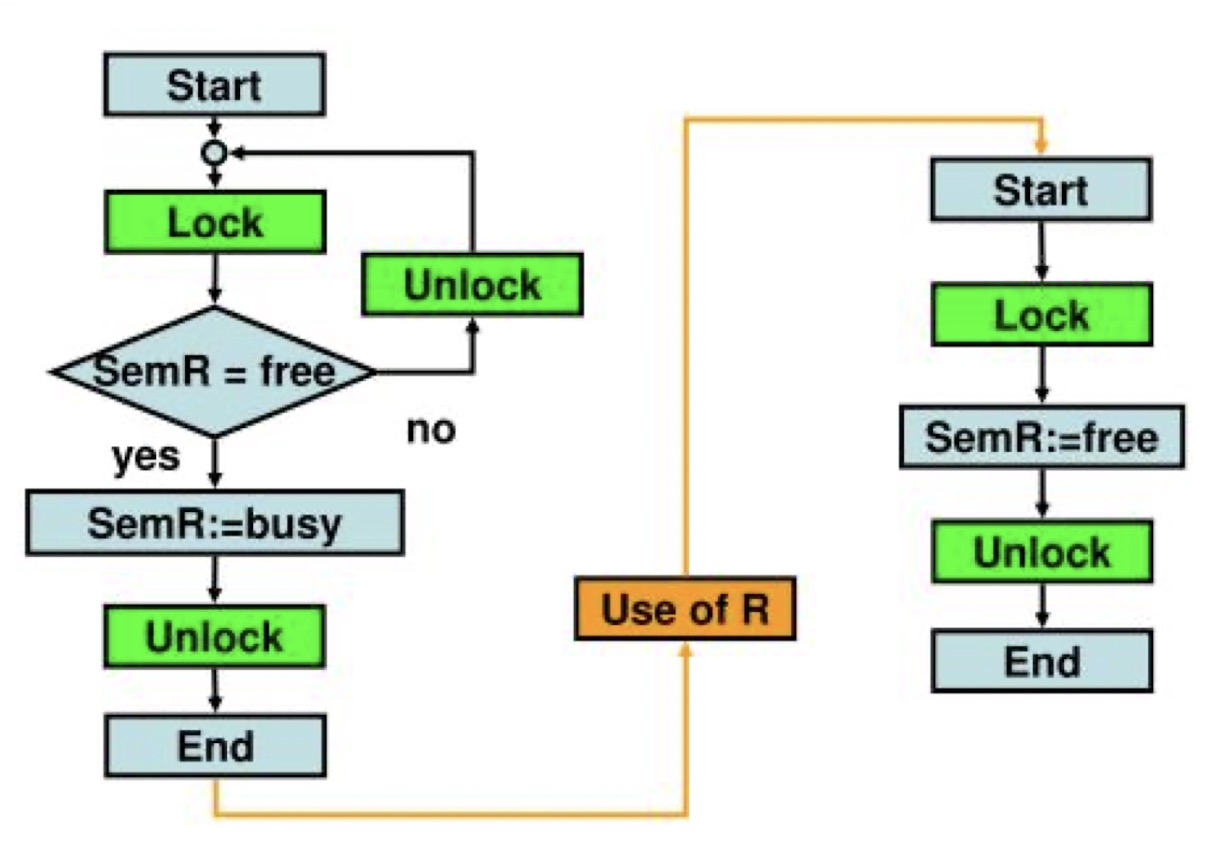
\includegraphics[width=0.5\linewidth]{assets/semaphore.jpg}
    \caption{Visualizzazione di un semaforo}
\end{figure}
